\documentclass[12pt, a4paper, titlepage, table]{article}
\usepackage{pdfpages}
\usepackage[utf8]{inputenc}
\usepackage[T1]{fontenc}
\usepackage{titlesec}
\usepackage[french]{babel}
\usepackage{caption}
\usepackage{float}
\usepackage{graphicx}
\usepackage[inner=2cm, outer=2cm, top=2cm, bottom=2cm]{geometry}
\usepackage[T1]{fontenc}
\usepackage{times}
\usepackage{xr} 
\usepackage{multirow}
\usepackage{amsmath}
\usepackage{array}
\usepackage{booktabs}
\usepackage{tabularx}
\usepackage{ragged2e}
\usepackage{adjustbox}

\begin{document}
	\label{document}
	\title{Etude de l'insertion professionnelle des diplômés de l'université (DUT, Licence Pro, MASTER LMD et Master ENS)}
	\author{Sébastien Mertès}
	\date{\today}
	\maketitle
	\renewcommand{\thesection}{\arabic{section}.}
	\renewcommand{\thesubsection}{\thesection\arabic{subsection}}
	\renewcommand{\tablename}{Tableau}
	\renewcommand{\abstractname}{Résumé}
	\captionsetup[table]{font={small}}
	\setlength{\parindent}{0pt}
	\captionsetup{labelfont=bf, font=small}
	\tableofcontents
	\newcolumntype{C}{>{\RaggedRight\arraybackslash}X}
	\newpage
	
\section{Introduction}
	
\section{Présentation des données}
	Nous avons 3 jeux de données représentant respectivement les informations concernant l'évaluation de l'insertion professionnelle sur le marché du travail des diplômés universitaires en DUT, Licence Professionnelle, Master LMD (Licence-Master-Doctorat) et Master ENS (Enseignement) de toutes les disciplines. 
	
	Ces données ont été collectées 18 mois et 30 mois après l'obtention du diplôme des sessions  2013 à 2019. Ainsi l'enquête a commencé en décembre 2015, pour s'achever en décembre 2021.
	
	Les données collectées regroupent, par niveau de diplôme, les disciplines, le taux d'insertion, le salaire brut et net estimé, le pourcentage des types de contrat professionnel (CDI, CDD, intérimaire etc...) ainsi que les secteurs d'activité, les professions et le type d'entreprises.
	
	Les tableaux 1 à 5 décrivent les différentes variables utilisées pour cette étude et le taux en pourcentage de valeurs manquantes de chaque modalité pour les les différentes catégories.
	
	Le Tableaux 1, présente la liste des diplômes universitaires pour les DUT, Licence Professionnelle et MASTERS.
	Les MASTERS sont distingués par le MASTER LMD et le MASTER ENS. 
	
	Les disciplines sont indiquées aussi bien individuellement (Informatique, histoire, droit, psychologie etc..), que par des ensembles de disciplines (Formations juridiques, économiques et de gestion, Sciences humaines et sociales etc...). L'ensemble de toutes les disciplines par niveau de diplôme est aussi indiqué (Ensemble MASTERS LMD, Ensemble des départements d'IUT etc...).   
	
	
	
\newpage

\begin{table}[H]
	\centering
	\begin{adjustbox}{max width=\textwidth}
		\begin{tabularx}{\linewidth}{|l|C|}
			\hline
			\multicolumn{1}{|c|}{\textbf{Diplôme}} & \multicolumn{1}{c|}{\textbf{Définition}} \\
			\hline
			DUT & Diplôme Universitaire de Technologie. Formation de 2 ans axée sur des compétences techniques et pratiques. \\
			\hline
			LICENCE PRO & Licence professionnelle. Programme de 1 an après un DUT ou une Licence, offrant une spécialisation professionnelle. \\
			\hline
			MASTER ENS & Master Enseignement. Diplôme permettant de devenir enseignant dans le système éducatif français. \\
			\hline
			MASTER LMD & Système européen d'enseignement supérieur avec niveaux de Licence, Master et Doctorat. \\
			\hline
		\end{tabularx}
	\end{adjustbox}
	\caption{Nom de la variable catégorielle et ses modalités concernant les diplômes universitaires}
	\label{tab:diplomes}
\end{table}

\begin{table}[H]
	\centering
	\begin{adjustbox}{max width=\textwidth}
	\begin{tabularx}{\linewidth}{|l|C|}
		\hline
		\multicolumn{1}{|c|}{\textbf{Discipline}} & \multicolumn{1}{c|}{\textbf{Ensemble}} \\
		\hline
		Autres sciences humaines et sociales & Ensemble Licence professionnelle \\
		\hline
		Autres formations juridiques, économiques et de gestion & Ensemble formations juridiques, économiques et de gestion \\
		\hline
		Sciences de la vie et de la terre & Ensemble des départements d'IUT \\
		\hline
		Psychologie & Ensemble sciences humaines et sociales \\
		\hline
		Information communication & Ensemble sciences, technologies et santé \\
		\hline
		Lettres, langues, arts & Autres sciences, technologies et santé \\
		\hline
		Sciences de l'ingénieur & Ensemble Masters LMD (hors Masters enseignement et hors Dauphine et Antilles-Guyane) \\
		\hline
		Histoire-géographie & Ensemble Masters LMD (hors Masters enseignement) \\
		\hline
		Droit & \\
		\hline
		Informatique & \\
		\hline
		Gestion & \\
		\hline
		Sciences fondamentales & \\
		\hline
		Économie & \\
		\hline
		Masters enseignement & \\
		\hline
	\end{tabularx}
	\end{adjustbox}
	\caption{Liste des disciplines et ensembles}
	\label{tab:disciplines}
\end{table}


\begin{table}[H]
	\centering
	\begin{tabularx}{\textwidth}{|X|c|}
		\hline
		\textbf{Contrat} & \textbf{\%} \\
		\hline
		Prof. libérale, indépendant, chef d’entreprise & 8.1 \\
		\hline
		Fonctionnaire & 8.1 \\
		\hline
		CDI & 8.1 \\
		\hline
		CDI de chantier ou CDI de mission & 8.8 \\
		\hline
		Contrat spécifique au doctorat & 10.5 \\
		\hline
		CDD & 8.1 \\
		\hline
		Vacataire & 8.1 \\
		\hline
		Intérimaire & 8.1 \\
		\hline
		Intermittent du spectacle & 8.1 \\
		\hline
		Contrat de professionnalisation & 8.1 \\
		\hline
		Emplois aidés (Contrat Initiative Emploi…) & 8.1 \\
		\hline
		Volontariat international & 8.1 \\
		\hline
	\end{tabularx}
	\caption{Pourcentage de valeurs manquantes des différents types de contrat}
	\label{tab:contrats_pourcentage}
\end{table}

\begin{table}[H]
	\centering
	\begin{tabularx}{\textwidth}{|X|c|}
		\hline
		\textbf{Entreprise} & \textbf{\%} \\
		\hline
		Vous-même & 11.0 \\
		\hline
		La fonction publique (d'etat, territoriale ou hospitalière) & 11.0 \\
		\hline
		Une entreprise privée & 11.0 \\
		\hline
		Une entreprise publique & 11.0 \\
		\hline
		Une association & 11.0 \\
		\hline
		Une personne exerçant une profession libérale ou un indépendant & 11.0 \\
		\hline
		Organisation internationale ou une institution de l'Union européenne & 11.5 \\
		\hline
		Société d'économie mixte & 11.4 \\
		\hline
		Un particulier & 11.0 \\
		\hline
	\end{tabularx}
	\caption{Pourcentage de valeurs manquantes par type d'entreprise}
	\label{tab:entreprise_pourcentage}
\end{table}


\begin{table}[H]
	\centering
	\begin{tabularx}{\textwidth}{|X|c|}
		\hline
		\textbf{Secteur} & \textbf{\%} \\
		\hline
		Agriculture, sylviculture et pêche & 7.1 \\
		\hline
		Industries (manufacturières, extractives et autres) & 7.1 \\
		\hline
		Construction & 7.1 \\
		\hline
		Activités immobilières & 7.4 \\
		\hline
		Commerce, transports, hébergement et restauration & 7.1 \\
		\hline
		Information et communication & 7.1 \\
		\hline
		Activités financières et d’assurance & 7.1 \\
		\hline
		Activités spécialisées, scientifiques et techniques & 7.1 \\
		\hline
		Activités de services administratifs et de soutien & 7.1 \\
		\hline
		Enseignement & 7.1 \\
		\hline
		Administration publique (hors enseignement) & 7.1 \\
		\hline
		Santé humaine et action sociale & 7.1 \\
		\hline
		Arts, spectacles et activités récréatives & 7.1 \\
		\hline
		Autres activités de service & 7.1 \\
		\hline
	\end{tabularx}
	\caption{Pourcentage de valeurs manquantes par secteur}
	\label{tab:secteurs_pourcentage}
\end{table}

\begin{table}[H]
	\centering
	\begin{tabularx}{\textwidth}{|X|c|}
		\hline
		\textbf{Profession} & \textbf{\%} \\
		\hline
		Agriculteur & 11.2 \\
		\hline
		Artisan, commerçant, chef d'entreprise & 11.1 \\
		\hline
		Profession libérale & 11.1 \\
		\hline
		Personnel de catégorie A de la fonction publique & 10.2 \\
		\hline
		Ingénieur, cadre, professions libérales, professions intellectuelles supérieures & 10.2 \\
		\hline
		Personnel de catégorie B de la fonction publique & 10.2 \\
		\hline
		Emploi de niveau intermédiaire : technicien, agent de maîtrise, etc. & 10.2 \\
		\hline
		Personnel de catégorie C de la fonction publique & 10.2 \\
		\hline
		Manœuvre, ouvrier & 10.2 \\
		\hline
		Employé de bureau, de commerce, personnel de service & 5.3 \\
		\hline
	\end{tabularx}
	\caption{Pourcentage de valeurs manquantes par profession}
	\label{tab:professions_pourcentage}
\end{table}


\section{Les types de contrats après l'obtention du diplôme}

	\subsection{Répartion des contrats à 18 et 30 mois après l'obtention du diplôme}
		\begin{figure}[H]
			\centering
			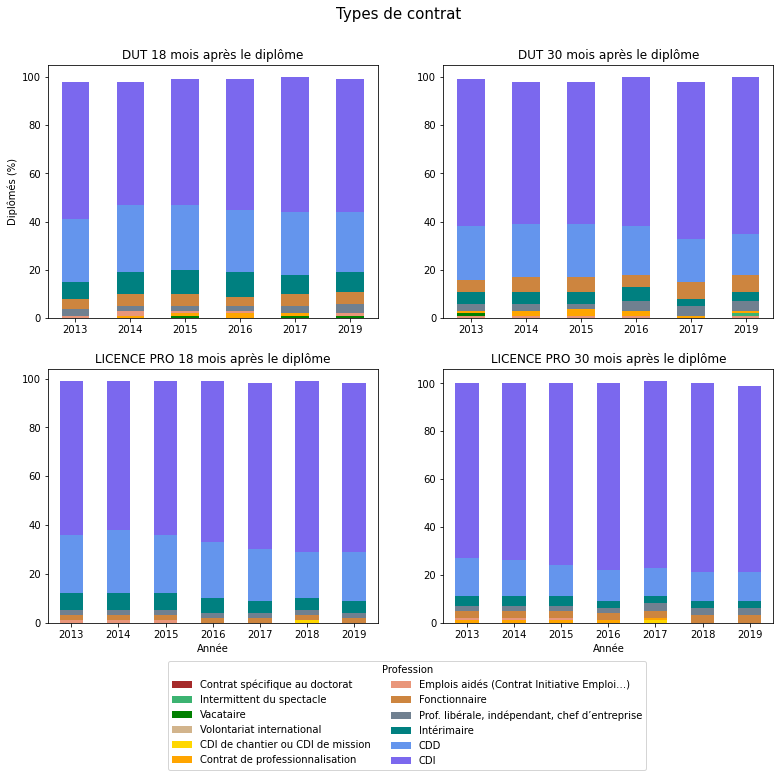
\includegraphics[width=1\textwidth]{../graphs/repartition_contrats_situation_1.png}
			\captionof{figure}{\textbf{Répartition des contrats à 18 et 30 mois après l'obtention du diplôme}}
		\end{figure}
	
		\begin{figure}[H]
			\centering
			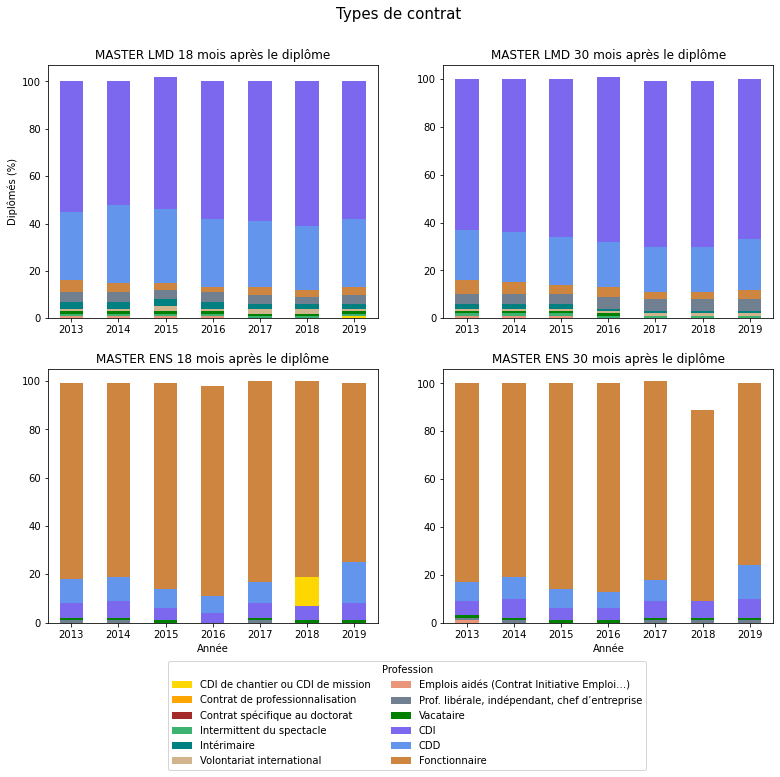
\includegraphics[width=1\textwidth]{../graphs/repartition_contrats_situation_2.png}
			\captionof{figure}{\textbf{Répartition des contrats à 18 et 30 mois après l'obtention du diplôme}}
		\end{figure}

\section{Les professions après l'obtention du diplôme}

	\subsection{Répartition des professions à 18 et 30 mois après l'obtention du diplôme}
		\begin{figure}[H]
			\centering
			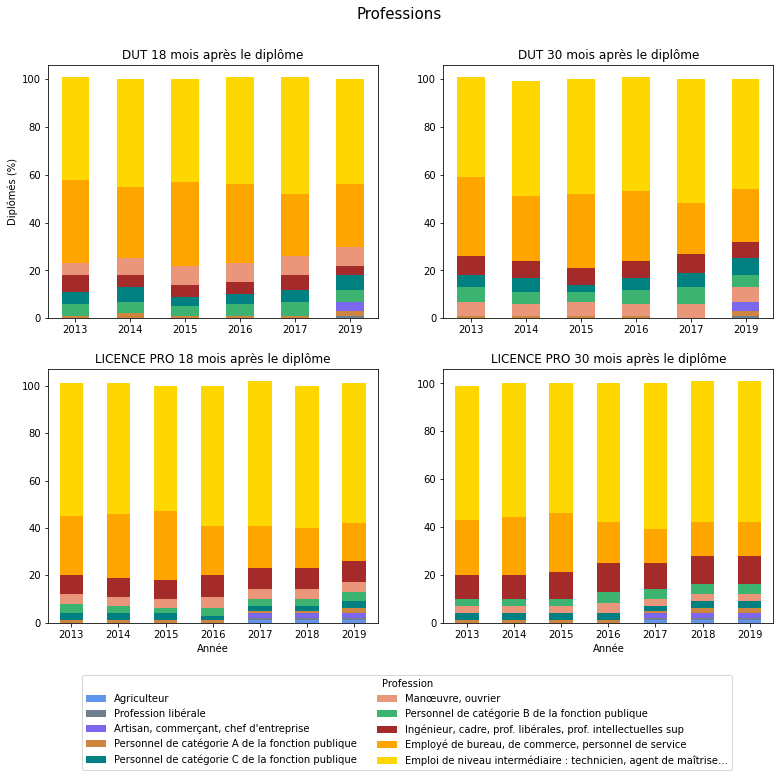
\includegraphics[width=1\textwidth]{../graphs/repartition_professions_situation_1.png}
			\captionof{figure}{\textbf{Répartition des professions à 18 et 30 mois après l'obtention du diplôme (DUT-Licence pro)}}
		\end{figure}
	
		\begin{figure}[H]
			\centering
			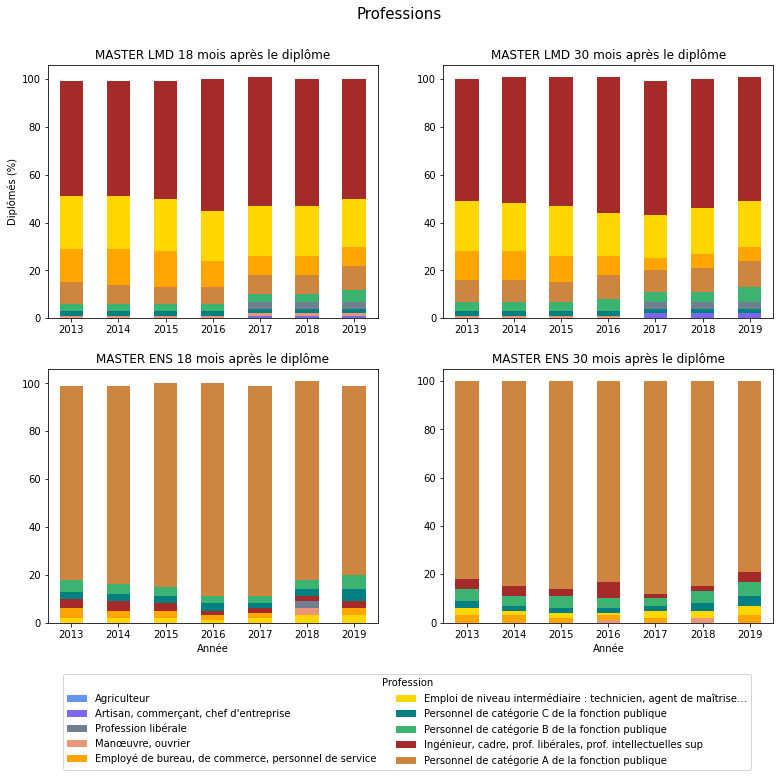
\includegraphics[width=1\textwidth]{../graphs/repartition_professions_situation_2.png}
			\captionof{figure}{\textbf{Répartition des professions à 18 et 30 mois après l'obtention du diplôme (Masters)}}
		\end{figure}


\section{Secteurs d'activité après l'obtention du diplôme}
	Les données 18 mois après l'obtention du diplôme étant manquantes, nous indiquons dans la Figure 5, le pourcentage des secteurs d'activité dans lesquels les diplômés se sont insérés 30 mois après son obtention. 

	\begin{figure}[H]
		\centering
		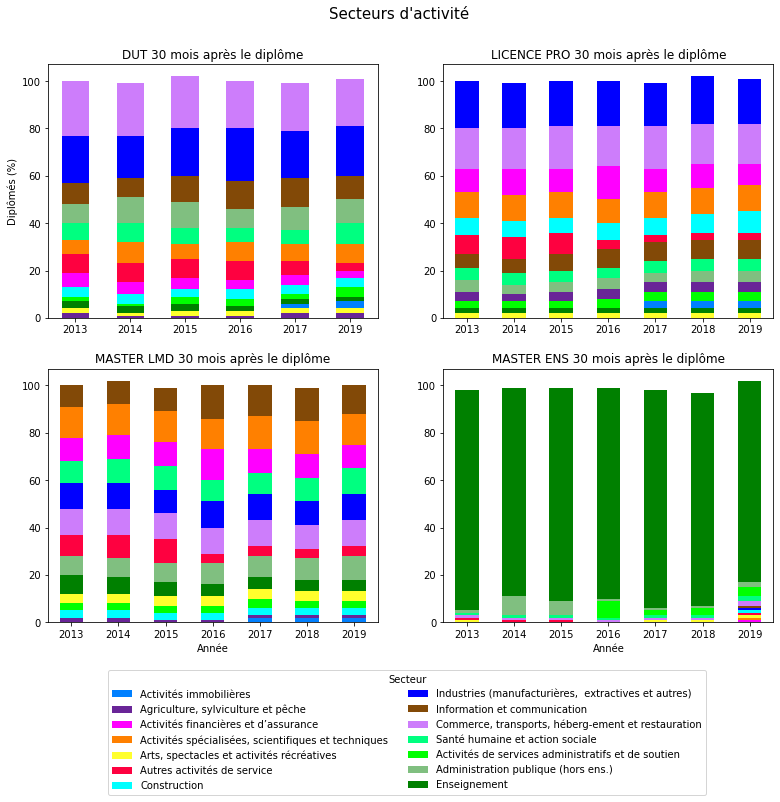
\includegraphics[width=1\textwidth]{../graphs/repartition_secteurs_situation.png}
		\captionof{figure}{\textbf{Répartition des secteurs à 18 et 30 mois après l'obtention du diplôme}}
	\end{figure}

\section{Taux d'insertion dans les emplois stables}

Le taux d’insertion est défini comme étant le pourcentage de diplômés occupant un emploi, quel qu’il soit, sur l’ensemble des diplômés présents sur le marché du travail. Il est calculé sur les diplômés de nationalité française, issus de la formation initiale, entrés immédiatement et durablement sur le marché du travail après l’obtention de leur diplôme en 2013, 2014, 2015, 2016, 2017, 2018 ou 2019.


\begin{figure}[H]
	\centering
	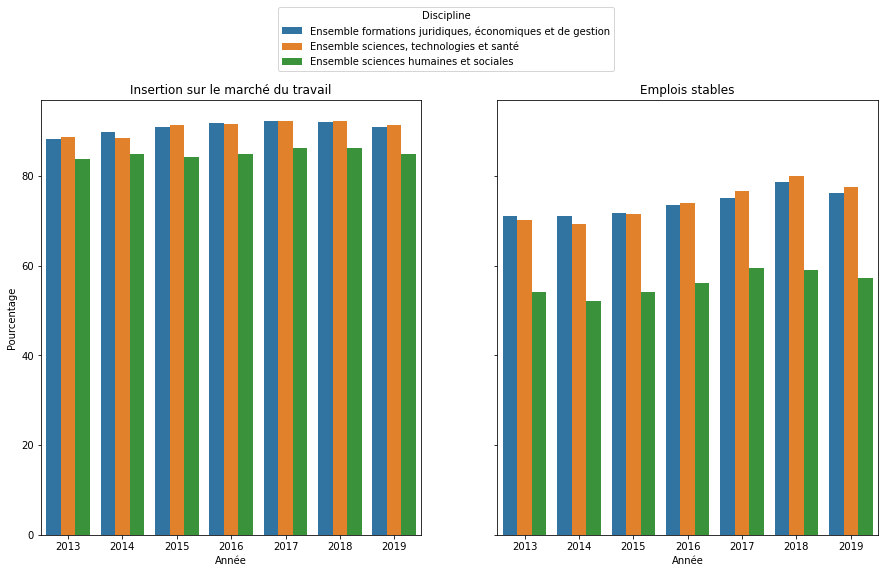
\includegraphics[width=1\textwidth]{../graphs/insertion_emploi_stable.png}
	\captionof{figure}{\textbf{Taux d'insertion sur le marché du travail et d'emplois stables}}
\end{figure}

\section{Salaires}
L’information collectée sur le salaire porte sur le salaire net, primes comprises. Les salaires affichés correspondent aux valeurs médianes sur les emplois à temps plein. A partir de ces valeurs, on estime un salaire brut annuel, sur la base d’un taux forfaitaire de passage du net au brut de 1,3 (donnée moyenne constatée sur les salaires du secteur privé).
L’enquête a été menée par les universités dans le cadre d’une charte dont les dispositions visent à garantir la comparabilité des résultats entre les établissements. La coordination d’ensemble et l’exploitation de l’enquête sont prises en charge par le ministère en charge de l'Enseignement supérieur et de la Recherche.

\end{document}